\FloatBarrier
\section{Nonlinear Model Predictive Control}
\label{sec::22_nmpc}
At the heart of nonlinear model predictive control stands sequential quadratic programming. Prior to the actual problem formulation, one needs to understand how sequential quadratic programming can be used to solve nonlinear optimization problems. One will then come to recognize that if one can find a canonical formulation of the problem, it will become possible to apply sequential quadratic programming to it. The next section - Sequential Quadratic Programming, will therefore shortly introduce the reader to the desired method that will be used to solve the nonlinear optimization problem, while the subsequent section - Canonical Formulation of Nonlinear Model Predictive Control, will then explain how to fit humanoid walking into this framework.
\FloatBarrier
\subsection{Sequential Quadratic Programming}
\label{sec::221_sqp}
Sequential quadratic programming is a powerful concept to solve nonlinearly constrained optimization problems. The nonlinear programming problem to be solved is of the form
\begin{align}
	\min_{\bm{x}}\, &\frac{1}{2}f(\bm{x})
	\label{eq::221_objective}\\
	\text{subject to: } &\bm{h}(\bm{x}) = \bm{0}\\
	&\bm{g}(\bm{x}) \leq \bm{0},
\end{align}
where $f:\,\mathbb{R}^N\rightarrow\mathbb{R}$, $\bm{h}:\,\mathbb{R}^N\rightarrow\mathbb{R}^M$, and $\bm{g}:\,\mathbb{R}^N\rightarrow\mathbb{R}^P$ \cite{boggs1995sequential}. These problems arise in a variety of applications in science and include quadratic problems as special cases. The great strength of sequential quadratic programming is its ability to solve problems with nonlinear constraints, and its basic idea is to model nonlinear programming at an approximate solution $\bm{x}_k$ by a quadratic subproblem, so to find a solution to this subproblem, in order to construct a better approximation $\bm{x}_{k+1}$. Now given an objective function $f(\bm{x})$ represents a sum of squares, the problem at hand turns into a nonlinear least squares problem, and the minimization can be expressed in terms of a Gauss-Newton method \cite{schittkowski1988solving}. That is, given an objective function $f(\bm{x}) = \bm{F}(\bm{x})^T\bm{F}(\bm{x})$, where $\bm{F}=\left(f_1,...,f_l\right)^T$, one can apply a quasi Gauss-Newton method as follows
\begin{align}
	\nabla^2f(\bm{x})\Delta\bm{x} + \nabla f(\bm{x}) = 0,
	\label{eq::221_quasi_gn}
\end{align}
where the gradient and the Hessian matrix are given as
\begin{align}
	\nabla f(\bm{x}) &= \nabla \bm{F}(\bm{x})\bm{F}(\bm{x}) \\
	\nabla^2 f(\bm{x}) &= \nabla \bm{F}(\bm{x})\nabla\bm{F}(\bm{x})^T + \bm{B}(\bm{x}).
\end{align}
Therein, $\bm{B}(\bm{x}) = \sum_1^lf_i(\bm{x})\nabla^2f_i(\bm{x})$. If $\bm{x}$ is now sufficiently close to an optimal solution $\bm{x}^*$, such that $\bm{F}(\bm{x}^*) = \left(f_1(\bm{x}^*),...,f_l(\bm{x}^*)\right)^T=\bm{0}$, one can neglect $\bm{B}(\bm{x^*})$, which turns equation \ref{eq::221_quasi_gn} into the previously stated Gauss-Newton minimization problem
\begin{align}
	\min_{\Delta\bm{x}}\,||\nabla\bm{F}(\bm{x_k})^T\Delta\bm{x}+\bm{F}(\bm{x}_k)||^2_2,
	\label{eq::221_gn_min}
\end{align}
where a new iterate is obtained by $\bm{x}_{k+1}=\bm{x}_k + \alpha_k\Delta \bm{x}$ with an appropriate step length parameter $\alpha_k$. This is because equation \ref{eq::221_quasi_gn} defines the normal equations of equation \ref{eq::221_gn_min}. The presented approach assures quadratic convergence, when starting sufficiently close to an optimal solution. The next section will explain how to apply this concept to control the zero moment point of a linear inverted pendulum in a balanced manner.
\FloatBarrier
\subsection{Canonical Formulation of Nonlinear Model Predictive Control}
Not only shall a humanoid robot keep dynamic balance in terms of the zero moment point, which was derived in equations \ref{eq::211_zmp_x} and \ref{eq::211_zmp_y}, but further shall this be assured for future time steps that are yet ahead. The underlying model predictive control got first introduced in \cite{kajita2003biped}, and is based upon a linear time-stepping scheme, which integrates the current jerk of the center of mass iteratively, so to estimate its future position. The linear time-stepping scheme will briefly present it in the following section.
\FloatBarrier
\subsection{Linear Time-Stepping Scheme}
Suppose that the center of mass' jerk $\dddot{c}_k$ at time step $t_k$ is constant, then given the current acceleration $\ddot{c}_k$, one can obtain the acceleration $\ddot{c}_{k+1}$ at time step $t_{k+1}$ by simple integration. The same can be done for the velocity and position, which yields
\begin{align}
	c_{k+1} &= \frac{T^3}{6}\dddot{c}_k+\frac{T^2}{2}\ddot{c}_k+T\dot{c}_k+c_k\\
	\dot{c}_{k+1} &= \frac{T^2}{2}\dddot{c}_k+T\ddot{c}_k+\dot{c}_k\\
	\ddot{c}_{k+1} &= T\dddot{c}_{k} + \ddot{c}_k,
\end{align}
where $T = t_{k+1}-t_k$. One can rewrite this in compact form by
\begin{align}
	&\bm{c}_{k+1} = \bm{A}\bm{c}_k + \bm{B}\dddot{c}_k \\
	&\bm{c}_{k+1} = \begin{pmatrix}
	c_{k+1} \\
	\dot{c}_{k+1} \\
	\ddot{c}_{k+1}
	\end{pmatrix},\,\,
	\bm{A} = \begin{pmatrix}
	1 & T & \frac{T^2}{2} \\
	0 & 1 & T \\
	0 & 0 & 1
	\end{pmatrix},\,\,
	\bm{B} = \begin{pmatrix}
	\frac{T^3}{6} \\
	\frac{T^2}{2} \\
	T
	\end{pmatrix}
	\label{eq::223_ltss}
\end{align}
Now by recursion, one obtains the positions, velocities, and accelerations for $n$ future time steps via
\begin{align}
	\bm{c}_{k+n} = \bm{A}^n\bm{c}_k\sum_{i=1}^n \bm{A}^{i-1}\bm{B}\dddot{c}_{k+n-i},
	\label{eq::223_preview}
\end{align}
where $n\in[1,N]$. Altogether one has
\begin{align}
	\bm{A}^n = \begin{pmatrix}
	1 & nT & n^2\frac{T^2}{2} \\
	0 & 1 & nT \\
	0 & 0 & 1
	\end{pmatrix},\,\,
	\bm{A}^n\bm{B} = \begin{pmatrix}
	(1+3n+3n^2)T^3/6 \\
	(1+2n)T^2/2 \\
	T
	\end{pmatrix}.
	\label{eq::223_preview_mat}
\end{align}
The amount of time $NT$ by which the linear time-stepping scheme predicts into the future, is called the preview horizon. If the single entries of $\bm{c}_{k+n}$ are now concatenated for all $n\in[1,N]$ into one expression, one can relate the initial states $\bm{c}_k$ to the states on the preview horizon in an even more compact form. With the concatenations
\begin{align}
	\bm{C}_{k+1}=\begin{pmatrix}
	c_{k+1}\\
	\vdots\\
	c_{k+N}
	\end{pmatrix},\,\,
	\dot{\bm{C}}_{k+1}=\begin{pmatrix}
	\dot{c}_{k+1}\\
	\vdots\\
	\dot{c}_{k+N}
	\end{pmatrix},\,\,
	\ddot{\bm{C}}_{k+1}=\begin{pmatrix}
	\ddot{c}_{k+1}\\
	\vdots\\
	\ddot{c}_{k+N}
	\end{pmatrix},\,\,
	\dddot{\bm{C}}_{k}=\begin{pmatrix}
	\dddot{c}_{k}\\
	\vdots\\
	\dddot{c}_{k+N-1}
	\end{pmatrix},
\end{align}
one obtains 
\begin{align}
	\bm{C}_{k+1} &= \bm{P}_{ps} \bm{c}_k + \bm{P}_{pu}\dddot{\bm{C}}_k
	\label{eq::223_ckp1}\\
	\dot{\bm{C}}_{k+1} &= \bm{P}_{vs} \bm{c}_k + \bm{P}_{vu}\dddot{\bm{C}}_k
	\label{eq::223_dckp1}\\
	\ddot{\bm{C}}_{k+1} &= \bm{P}_{as} \bm{c}_k + \bm{P}_{au}\dddot{\bm{C}}_k,
	\label{eq::223_ddckp1}
\end{align}
where the new matrices are given by 
\begin{align}
	\bm{P}_{ps} &= \begin{pmatrix}
	1 & T & T^2/2 \\
	\vdots & & \vdots \\
	1 & nT & n^2T^2/2
	\end{pmatrix},\,\,
	\bm{P}_{pu} = \begin{pmatrix}
	T^3/6 & \dots & 0 \\
	\vdots & \ddots & \vdots \\
	(1+3n+3n^2)T^2/6 & \dots & T^3/6
	\end{pmatrix} \\
	\bm{P}_{vs} &= \begin{pmatrix}
	0 & 1 & T \\
	\vdots & & \vdots \\
	0 & 1 & nT
	\end{pmatrix},\,\,
	\bm{P}_{vu} = \begin{pmatrix}
	T^2/2 & \dots & 0 \\
	\vdots & \ddots & \vdots \\
	(1+2n)/T^2/2 & \dots & T^2/2
	\end{pmatrix} \\
	\bm{P}_{as} &= \begin{pmatrix}
	0 & 0 & 1 \\
	\vdots  &  & \vdots \\
	 0 & 0 & 1
	\end{pmatrix},\,\,
	\bm{P}_{au}\begin{pmatrix}
	T & \dots & 0 \\
	\vdots & \ddots & \vdots \\
	T & \dots & T
	\end{pmatrix}.
\end{align}
If one now additionally considers the relation of the zero moment point and the center of mass, which was obtained earlier in equations \ref{eq::211_zmp_x} and \ref{eq::211_zmp_y}, one can further relate the current center of mass state to the zero moment point on the preview horizon by
\begin{align}
	\bm{Z}_{k+1} &= \bm{C}_{k+1} - \frac{c_z}{g}\ddot{\bm{C}}_{k+1} \\
	&= \left(\bm{P}_{ps}-\frac{c_z}{g}\bm{P}_{as}\right)\bm{c}_k + \left(\bm{P}_{pu}-\frac{c_z}{g}\bm{P}_{au}\right)\ddddot{\bm{C}}_k = \bm{P}_{zs} \bm{c}_k + \bm{P}_{zu}\dddot{\bm{C}}_k,
	\label{eq::223_zmp}
\end{align}
where the new matrices are given by 
\begin{align}
	\bm{P}_{zs} &= \begin{pmatrix}
	1 & T & T^2/2 - c_z/g \\
	\vdots & & \vdots \\
	1 & nT & n^2T^2/2 - c_z/g
	\end{pmatrix} \\ 
	\bm{P}_{zu} &= \begin{pmatrix}
	T^3/6 - Tc_z/g & \dots & 0 \\
	\vdots & \ddots & \vdots \\
	(1+3n+3n^2)T^3/6 - Tc_z/g & \dots & T^3/6-Tc_z/g
	\end{pmatrix}.
\end{align}
The expressions for the preview horizon now allow one to formulate an objective function that takes the robot's dynamic balance for future time steps into account, which in turn results in actions being taken that already take future predictions of the system's dynamics into account. The cost function, therefore, is described in the next section.
\FloatBarrier
\subsection{The Objective Function}
To create an objective function, as the one already outlined in section \ref{sec::221_sqp}, one can put together squared $L^2$-norm objectives, which account for a desired reference center of mass velocity $\dot{\bm{C}}_{k+1}^\text{ref}$, a balanced footstep placement $\textbf{F}_{k+1}$ close to the zero moment point $\bm{Z}_{k+1}$, and a smooth motion for which the center of mass jerk $\dddot{\bm{C}}_{k+1}$ enters as a regularization. The objective function itself is similar to the one first introduced in \cite{herdt2010online}, but additionally takes the center of mass' rotation around the z-axis into account, and it can be written down as follows
\begin{align}
	\min_{\bm{U}_k} &\frac{\alpha}{2}||\dot{\bm{C}}^x_{k+1} - \dot{\bm{C}}_{k+1}^{x,\text{ref}}||_2^2 + \frac{\alpha}{2}||\dot{\bm{C}}^y_{k+1} - \dot{\bm{C}}_{k+1}^{y,\text{ref}}||_2^2 
	\label{eq::224_dcxy}\\
	&\frac{\alpha}{2}||\bm{E}_L\dot{\bm{F}}^{\theta,L}_{k+1} - \dot{\bm{C}}_{k+1}^{\theta,\text{ref}}||_2^2 + 	\frac{\alpha}{2}||\bm{E}_R\dot{\bm{F}}^{\theta,R}_{k+1} - \dot{\bm{C}}_{k+1}^{\theta,\text{ref}}||_2^2 
	\label{eq::224_dftheta} \\
	&\frac{\beta}{2}||\bm{Z}^x_{k+1}-\bm{F}^x_{k+1}||^2_2 + \frac{\beta}{2}||\bm{Z}^y_{k+1}-\bm{F}^y_{k+1}||^2_2 
	\label{eq::224_fxy}\\
	&\frac{\gamma}{2}||\dddot{\bm{C}}_{k+1}^x||^2_2 + \frac{\gamma}{2}||\dddot{\bm{C}}_{k+1}^y||^2_2	
	\label{eq::224_dddcxy}
\end{align}
Before addressing the foot placement therein in more detail, it is worth noting that the reference velocities are the commands, which later enter the control loop from figure \ref{fig::21_pg}. One sets them to be constant over the whole preview horizon and rotates them to the world frame  by considering the robot's current orientation. When considering that the foot cannot move once it is in contact with the ground, it becomes clear that the footstep placement must be very discrete in time. The number of steps $N_f$ that are planned for in advance is simply given by $NT/T_\text{step}$, where the duration of the preview horizon $NT$ is divided by the time it takes to perform a step $T_\text{step}$. But as already shown in equation \ref{eq::223_zmp}, and used in equation \ref{eq::224_fxy}, one requires balance on a finer timescale. Therefore, the foot placement $\tilde{\bm{F}}_k\in\mathbb{R}^{N_f\times1}$ is projected onto the temporal resolution of the center of mass' control variable by introducing the matrices $\bm{v}_{k+1}$, $\bm{V}_{k+1}$, and the current foot position $f_k$, which yields
\begin{align}
	\bm{F}_{k+1} = \bm{v}_{k+1}f_k + \bm{V}_{k+1}\tilde{\bm{F}}_k,
	\label{eq::224_feet}
\end{align}
where $\bm{v}_{k+1}$ is a $N\times1$ matrix, and $\bm{V}_{k+1}$ is a $N\times N_f$ matrix, and they are for example for $N_f = 3$ given by
\begin{align}
	\bm{v}_{k+1} = \begin{pmatrix}
	1 \\ 
	\vdots \\
	1 \\
	0 \\
	\vdots \\
	0 \\
	0 \\
	\vdots \\
	0
	\end{pmatrix},\,\, 
	\bm{V}_{k+1} = \begin{pmatrix}
	0 & 0 & 0\\
	\vdots & \vdots & \vdots \\
	0 & 0 & 0 \\
	0 & 1 & 0 \\
	\vdots & \vdots & \vdots \\
	0 & 1 & 0 \\
	0 & 0 & 1 \\
	\vdots & \vdots & \vdots \\
	0 & 0 & 1
	\end{pmatrix}
\end{align}
As the robot moves, the matrices change, in that the entries of $v_{k+1}$ are being shifted upwards by one index for every time step $T$, while the new entries at the bottom are set to be zero. All entries of $V_{k+1}$ are also shifted upwards, while the bottom right entry is set to one, but further are all entries of $V_{k+1}$ are being shifted to the left once all entries of $\bm{v}_{k+1}$ are zero. If all entries of $\bm{v}_{k+1}$ are zero, then $\bm{v}_{k+1}$ is replaced by the second column of $\bm{V}_{k+1}$. For example, for $N_f = 2$ and $N=6$ one has
\begin{align}
	\left(
	\begin{array}{c|c}
	\bm{v}_{k+1} & \bm{V}_{k+1}
	\end{array} 
	\right) =
	\left(
	\begin{array}{c|cc}
	1 & 0 & 0 \\
	0 & 1 & 0 \\
	0 & 1 & 0 \\ 
	0 & 1 & 0 \\
	0 & 0 & 1 \\
	0 & 0 & 1
	\end{array}\right) \rightarrow
	\left(
	\begin{array}{c|cc}
	1 & 0 & 0 \\
	1 & 0 & 0 \\
	1 & 0 & 0 \\ 
	0 & 1 & 0 \\
	0 & 1 & 0 \\
	0 & 1 & 0
	\end{array}\right) \rightarrow
	\left(
	\begin{array}{c|cc}
	1 & 0 & 0 \\
	1 & 0 & 0 \\
	0 & 1 & 0 \\ 
	0 & 1 & 0 \\
	0 & 1 & 0 \\
	0 & 0 & 1
	\end{array}\right)
	\label{eq::224_fs}
\end{align}
Now to ensure the rotation of the center of mass, one introduces equation \ref{eq::224_dftheta} to the objective function. The matrices $\bm{E}_{L/R}$ therein ensure that only the foot, which is currently not touching the ground, is rotated, the rotational velocity of the center of mass itself is then obtained by averaging over the left and the right foot. Hence $\bm{E}_{L/R}$ take the form
\begin{align}
	\bm{E}_L = \begin{pmatrix}
	1&&&&&&&& \\
	&\ddots&&&&&&& \\
	&&1&&&&&& \\
	&&&0&&&&& \\
	&&&&\ddots&&&& \\
	&&&&&0&&& \\
	&&&&&&1&& \\
	&&&&&&&\ddots& \\
	&&&&&&&&1 \\
	\end{pmatrix},\,\,
	\bm{E}_R = \bm{1} - \bm{E}_L
	\label{eq::224_fsm}
\end{align}
The diagonal entries therein just take the same form as a single column of $\bm{V}_{k+1}$, all other entries are zero. If one now takes equations \ref{eq::224_dcxy}-\ref{eq::224_dddcxy}, and replaces $\dot{\bm{C}}_{k+1}^{x/y}$, as well as $\dot{\bm{F}}_{k+1}^{\theta,L/R}$, by equation \ref{eq::223_dckp1}, and inserts equation \ref{eq::223_zmp} into the zero moment point on the preview horizon $\bm{Z}_{k+1}$, one obtains following relation 
\begin{align}
	\min_{\bm{U}_k} &\frac{1}{2}\bm{U_k}^T\bm{Q}_k\bm{U}_k + \bm{p}_k^T\bm{U}_k
	\label{eq::224_canqp} \\
	& \bm{U}_k = \begin{pmatrix}
	\bm{U}^{xy}_k & \bm{U}^\theta_k
	\end{pmatrix}^T\\	
	&\bm{U}^{xy}_k = \begin{pmatrix}
	\dddot{\bm{C}}^x_k & \tilde{\bm{F}}_k^x & \dddot{\bm{C}}_k^y & \tilde{\bm{F}}_k^y
	\end{pmatrix}^T\\
	&\bm{U}^\theta_k = \begin{pmatrix} \dddot{\bm{F}}_k^{\theta, L} & \dddot{\bm{F}}_k^{\theta, R} 
	\end{pmatrix}^T \\
	&\bm{Q}_k = \begin{pmatrix}
	\bm{Q}_k^{x} & \bm{0} & \bm{0} & \bm{0} \\
	\bm{0} & \bm{Q}_k^{y} & \bm{0} & \bm{0} \\
	\bm{0} & \bm{0} & \bm{Q}_k^L & \bm{0} \\ 
	\bm{0} & \bm{0} & \bm{0} & \bm{Q}_k^R
	\end{pmatrix}
	\label{eq::224_qk}\\
	& \bm{Q}_k^x = \bm{Q}_k^y = \begin{pmatrix}
		\alpha\bm{P}_{vu}^T\bm{P}_{vu}+\beta\bm{P}_{zu}^T\bm{P}_{zu}+\gamma\bm{1} & -\beta\bm{P}_{zu}^T\bm{V}_{k+1} \\
		-\beta\bm{V}_{k+1}^T\bm{P}_{zu} & \beta\bm{V}_{k+1}^T\bm{V}_{k+1}
	\end{pmatrix}\\
	& \bm{Q}_k^{L/R} = \begin{pmatrix}
		\alpha\bm{P}_{vu}^T\bm{E}_{L/R}^T\bm{E}_{L/R}\bm{P}_{vu}
	\end{pmatrix}\\
	&\bm{p}_k = \begin{pmatrix}
		\bm{p}_k^x \\
		\bm{p}_k^y \\
		\bm{p}_k^{L} \\
		\bm{p}_k^{R}
	\end{pmatrix} \\
	& \bm{p}_k^{x/y} = \begin{pmatrix}
		\alpha\bm{P}_{vu}^T(\bm{P}_{vs}\bm{c}_k^{x/y}-\dot{\bm{C}}_{k+1}^{x/y,\text{ref}}) + \beta\bm{P}_{zu}^T(\bm{P}_{zs}\bm{c}_k^{x/y}-\bm{v}_{k+1}f_k^{x/y})\\
		-\beta\bm{V}_{k+1}^T(\bm{P}_{zs}\bm{c}_k^{x/y}-\bm{v}_{k+1}f_k^{x/y})
	\end{pmatrix} \\
	& \bm{p}_k^{L/R} = \begin{pmatrix}
		\alpha\bm{P}_{vu}^T\bm{E}_{L/R}^T(\bm{E}_{L/R}\bm{P}_{vs}\bm{f}_k^{q,L/R}-\dot{\bm{C}}_{k+1}^{L/R,\text{ref}})
	\end{pmatrix}
\end{align}
where all squared $L^2$-norms were evaluated via $||\bm{a}-\bm{b}||^2_2 = (\bm{a}-\bm{b})^T(\bm{a}-\bm{b})$, and ordered correspondingly. All terms that do not depend on the control variable $\bm{U}_k$ got discarded. Equation \ref{eq::224_canqp} now represents the canonical formulation of the minimization problem from equation \ref{eq::221_objective}. The formulation itself minimizes the objective of keeping the zero moment point close to the center of the feet, but it does not assure that it never leaves the support polygon. Also, does it not consider the kinematic feasibility of the solution. Therefore, one has to introduce constraints on the free parameters of the optimal control problem, which are explained in the next section.
\FloatBarrier
\subsection{The Constraints}
There are constraints of different nature. The constraints first constraints, ensure dynamic balance in that they constrain the zero moment point to the support polygon of the feet. Secondly, the feasibility constraints force the feet positioning to a convex hull that describes kinematically feasible motions. Finally, the constraints which restrict the feet's relative velocity, and the feet's relative orientation, as well as the ones, which allow obstacle avoidance, are introduced.
\subsubsection{Balance Constraints} 
To ensure that the zero moment point stays within the support polygon (figure \ref{fig::225_foot_hull}), one sets up a system of linear equations, of which each describes a line that connects the polygon's edges $\bm{p}_i$. 
\begin{figure}[h!]
	\centering
	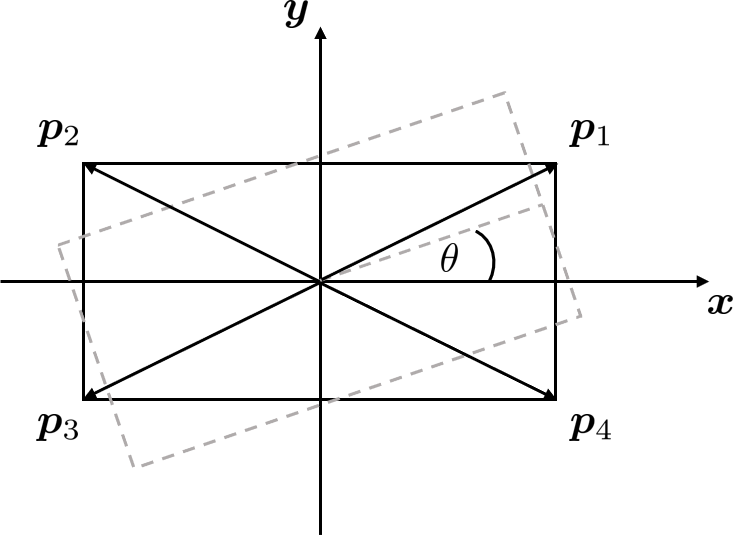
\includegraphics[scale=.5]{chapters/02_foundations_for_humanoid_walking/img/foot_convex_hull.png}
	\caption{The foot's support polygon, which is described by the position vectors $\bm{p}_i$.}
	\label{fig::225_foot_hull}
\end{figure}
A point $\bm{x}$ lies beneath the line that connects the edges if
\begin{align}
	\bm{A}^{L/R}\bm{x} \leq \bm{B}^{L/R},
	\label{eq::225_lin}
\end{align}
where the linear equations are defined by  $\bm{A}^{L/R}=\begin{pmatrix}
\bm{A}^{L/R,x}\,\bm{A}^{L/R,y}\end{pmatrix}\in\mathbb{R}^{N_{\text{edges}}\times2}$, and $\bm{B}^{L/R}\in\mathbb{R}^{N_{\text{edges}}\times1}$
\begin{align}
	\bm{A}^{L/R,x}[i] &= p^{L/R,y}_i-p^{L/R,y}_{i+1} \\
	\bm{A}^{L/R,y}[i] &= p^{L/R,x}_{i+1}-p^{L/R,x}_i \\
	\bm{B}^{L/R}[i] &= (p^{L/R,y}_i-p^{L/R,y}_{i+1})p^{L/R,x}_{i+1} + (p^{L/R,x}_{i+1}-p^{L/R,x}_i)p^{L/R,y}_{i+1}
\end{align}
Since one requires the zero moment point to lie inside the support polygon, $\bm{x}$ in equation \ref{eq::225_lin} is replaced by $\bm{R}_z(f_k^\theta)(\bm{z}_k-\bm{f}_k)$, with $\bm{z}_k=\begin{pmatrix}
z_k^x & z_k^y
\end{pmatrix}^T$, and $\bm{f}_k=\begin{pmatrix}
f_k^x & f_k^y
\end{pmatrix}^T$. This expression describes the zero moment point with respect to the foot frame, where $\bm{R}_z(f_k^\theta) = \begin{pmatrix}
\quad\cos f_k^\theta & \sin f_k^\theta \\
-\sin f_k^\theta& \cos f_k^\theta
\end{pmatrix}$ is an inverse rotation around the z-axis that adds non-linearities to the constraints. One can now extent the formalism to the whole preview horizon by utilizing equations \ref{eq::223_zmp} and \ref{eq::224_feet}. This leads to 
\begin{align}
	&\bm{D}_{k+1}(\bm{F}_{k+1}^{\theta})\begin{pmatrix}
		\bm{Z}_{k+1}^x - \bm{F}_{k+1}^x \\
		\bm{Z}_{k+1}^y - \bm{F}_{k+1}^y
	\end{pmatrix} \leq \bm{B}_{k+1} \\
	&\bm{D}_{k+1}(\bm{F}_{k+1}^{\theta})\begin{pmatrix}
		\bm{P}_{zs} \bm{c}_k^x + \bm{P}_{zu}\dddot{\bm{C}}_k^x - \bm{v}_{k+1}f_k^x-\bm{V}_{k+1}\tilde{\bm{F}}_{k+1}^x \\
		\bm{P}_{zs} \bm{c}_k^y + \bm{P}_{zu}\dddot{\bm{C}}_k^y - \bm{v}_{k+1}f_k^y-\bm{V}_{k+1}\tilde{\bm{F}}_{k+1}^y
	\end{pmatrix} \leq \bm{B}_{k+1}
	\label{eq::22_cop_hull}
\end{align}
where $\bm{D}_{k+1}\in\mathbb{R}^{N_\text{edges}N\times2N}$ depends on $\bm{F}_{k+1}^{\theta} = \bm{P}_{ps}f_k^\theta + \bm{P}_{pu}\bm{F}_{k+1}^\theta$, and holds all the linear equations on the whole preview horizon 
\begin{align}
\bm{D}_{k+1} = \begin{pmatrix}
	\bm{A}^{L/R,x}\bm{R}_z(f_{k+1}^\theta)&                  &\bm{0}                 &\bm{A}^{L/R,y}\bm{R}_z(f_{k+1}^\theta)&      &\bm{0} \\
	                  &\ddots            &                  &                  &\ddots& \\
	\bm{0}                 &                  &\bm{A}^{L/R,x}\bm{R}_z(f_{k+N}^\theta)&\bm{0}                 &      &\bm{A}^{L/R,y}\bm{R}_z(f_{k+N}^\theta)
\end{pmatrix},
\label{eq::225_rot1}
\end{align}
and $\bm{B}_{k+1}=\begin{pmatrix} \bm{B}^{L/R} & \dots & \bm{B}^{L/R}\end{pmatrix}^T$. Whether the left foot's or the right foot's convex hull is chosen depends on the support foot at the respective preview interval $k$. Equation \ref{eq::22_cop_hull} can now be expressed in terms of the free variables $\bm{U}_k$ by
\begin{align}
	\bm{D}_{k+1}\begin{pmatrix}
		\bm{P}_{zu} & -\bm{V}_{k+1} & \bm{0} & \bm{0}\\
		\bm{0} & \bm{0} & \bm{P}_{zu} & -\bm{V}_{k+1}
	\end{pmatrix}\bm{U}_k^{xy} &\leq \bm{B}_{k+1} + \bm{D}_{k+1}\begin{pmatrix}
		-\bm{P}_{zs}\bm{c}_k^x + \bm{v}_{k+1}f_k^x\\
		-\bm{P}_{zs}\bm{c}_k^y + \bm{v}_{k+1}f_k^y
	\end{pmatrix} \\
	\bm{A}_{\text{zmp},k}(\bm{U}_k^\theta)\bm{U}_k^{xy} &\leq \overline{\bm{U}_{\text{zmp},k}},
	\label{eq::225_ineq_zmp}
\end{align}
where $\overline{\bm{U}_{\text{zmp},k}}$ defines the upper bounds. The above derivation delivers a nice framework, which can be used to express the feasibility constraints as well.
\subsubsection{Feasibility Constraints}
The feasibility constraints constrain the foot positioning to areas that the robot of interest can actually reach, which can again be defined as a set of linear inequalities, with the position vectors $\bm{p}_i$ that are shown in figure \ref{fig::225_foot_feasibility}. 
\begin{figure}[h!]
	\centering
	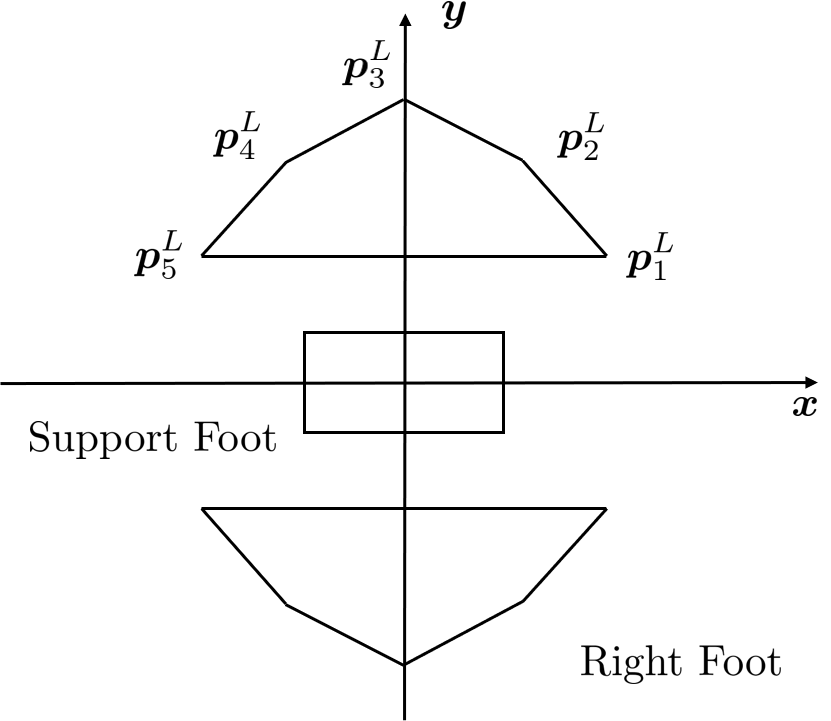
\includegraphics[scale=.5]{chapters/02_foundations_for_humanoid_walking/img/foot_constraints.png}
	\caption{The foot's feasibility polygon, which is described by the position vectors $\bm{p}_i$. The center is always defined by the current support foot's position, within the picture the support foot can therefore be the left as well as the right foot.}
	\label{fig::225_foot_feasibility}
\end{figure}
One can therefore just reuse the concept of equation \ref{eq::225_lin}, and replace $\bm{x}$ therein by the difference of the next foot position $\tilde{\bm{F}}_{k}\in\mathcal{R}^{N_f\times1}$, and the previous one $\tilde{\bm{F}}_{k-1} = \bm{S}_0\tilde{\bm{F}}_{k} + \bm{S}_1f_k$, where $\bm{S}_0 = \begin{pmatrix}0 & 0 \\ \textbf{I}_{N_f-1} & 0
\end{pmatrix}\in\mathcal{R}^{N_f\times N_f}$ simply shifts $\tilde{\bm{F}}_{k}$ down by one row, and $\bm{S}_1 = \begin{pmatrix}
1 \\ 0 \\ \vdots \\ 0
\end{pmatrix}\in\mathcal{R}^{N_f\times1}$. Altogether one has
\begin{align}
\begin{pmatrix}
\bm{A}_{k+1}^{x}&\bm{A}_{k+1}^{y}\end{pmatrix} 
\begin{pmatrix}
\tilde{\bm{F}}^x_{k} - \bm{S}_0\tilde{\bm{F}}^x_{k} - \bm{S}_1f^x_k\\
\tilde{\bm{F}}^y_{k} - \bm{S}_0\tilde{\bm{F}}^y_{k} - \bm{S}_1f^y_k
\end{pmatrix} &\leq \bm{B}_{k+1} \\
\begin{pmatrix}
\bm{0} & \bm{A}_{k+1}^{x}(\textbf{I}_{N_f}-\bm{S}_0) & \bm{0} & \bm{A}_{k+1}^{y}(\textbf{I}_{N_f}-\bm{S}_0)
\end{pmatrix}\bm{U}_k^{xy} &\leq \bm{B}_{k+1}+\begin{pmatrix}
\bm{S}_1f_k^x \\ \bm{S}_1f_k^x 
\end{pmatrix}\\
\bm{A}_{\text{foot},k}(\bm{U}_k^\theta)\bm{U}_k^{xy} &\leq \overline{\bm{U}_{\text{foot},k}},
\label{eq::225_ineq_foot}
\end{align}
where $\bm{A}_{k+1}^{x/y}=\begin{pmatrix}
	\bm{A}^{L/R,x/y}\bm{R}_z(f_{k}^\theta)& & \bm{0} \\
	&\ddots &\\
	\bm{0} &           &\bm{A}^{R/L,x/y}\bm{R}_z(f_{k+N_fN}^\theta)
\end{pmatrix}\in\mathbb{R}^{N_\text{edges}N\times N_f}$ has alternating linear inequalities $\bm{A}^{L/R,x/y}\rightarrow\bm{A}^{R/L,x/y}$ that correspond on the support foot, and so does $\bm{B_{k+1}}\in\mathbb{R}^{N_\text{edges}N\times1}$. 
\subsubsection{Relative Constraints}
By considering the maximum and minimum angle by which the feet are relatively oriented towards each other, one takes hardware limits into account. Furthermore, the restriction of the maximally allowed relative angular velocity decreases that variation of acceleration before the foot landing \cite{naveau2016reactive}. The constraints can be formulated as follows
\begin{align}
	-\bm{\theta}_\text{max}\leq\bm{F}_{k+1}^{L,\theta} - \bm{F}_{k+1}^{R,\theta} &\leq \bm{\theta}_\text{max} \\
	-\dot{\bm{\theta}}_\text{max}\leq\dot{\bm{F}}_{k+1}^{L,\theta} - \dot{\bm{F}}_{k+1}^{R,\theta} &\leq \dot{\bm{\theta}}_\text{max},
\end{align}
which can be expressed in terms of the free variables with equations \ref{eq::223_ckp1} and \ref{eq::223_dckp1} to find
\begin{align}
	-\bm{\theta}_\text{max}-\bm{P}_{ps}(f_k^L-f_k^R)&\leq \begin{pmatrix}
	\bm{P}_{pu} & -\bm{P}_{pu}
	\end{pmatrix}\bm{U}_k^\theta \leq \bm{\theta}_\text{max}-\bm{P}_{ps}(f_k^L-f_k^R) \\
	\underline{\bm{U}_{\text{ori},k}}&\leq \bm{A}_{\text{ori},k}\bm{U}_k^\theta \leq \overline{\bm{U}_{\text{ori},k}}\\
		-\dot{\bm{\theta}}_\text{max}-\bm{P}_{vs}(f_k^L-f_k^R)&\leq \begin{pmatrix}
	\bm{P}_{vu} & -\bm{P}_{vu}
	\end{pmatrix}\bm{U}_k^\theta \leq \dot{\bm{\theta}}_\text{max}-\bm{P}_{vs}(f_k^L-f_k^R)\\
	\underline{\bm{U}_{\text{dori},k}}&\leq \bm{A}_{\text{dori},k}\bm{U}_k^\theta \leq \overline{\bm{U}_{\text{dori},k}}.
	\label{eq::225_ineq_rot}
\end{align}
\subsubsection{Obstacle Constraints}
In contrast to similar methods like \cite{herdt2010walking}, the avoidance of convex obstacles is included, by requesting that the feet's positions must lie outside of circles $C = \{(p^x, p^y)\in\mathbb{R}^2 \,|\, (p^x-x_0)^2+(p^y-y_0)^2\leq R^2\}$, which define the obstacles, where $x_0$, and $y_0$ define the obstacle's center in world coordinates. This can be formulated by the free variables by
\begin{align}
	&(f_k^x-x_0)^2 + (f_k^y-y_0)^2 \geq (R + m)^2
	\label{eq::225_obstacle}\\
	&\bm{U}_k^{xy,T}\begin{pmatrix}
	\bm{0} & \textbf{I}_{N_f} & \bm{0}& \textbf{I}_{N_f}
	\end{pmatrix}\bm{U}_k^{xy} - \\&\begin{pmatrix}
	\bm{0} & \begin{pmatrix}
	2x_0 & \dots & 2x_0
	\end{pmatrix} & \bm{0} & \begin{pmatrix}
	2y_0 & \dots & 2y_0
	\end{pmatrix}
	\end{pmatrix} \bm{U}_k^{xy}\geq \begin{pmatrix}
	(R + m)^2-x_0^2-y_0^2 \\
	\vdots \\
	(R + m)^2-x_0^2-y_0^2
	\end{pmatrix}\\
	&\bm{U}_k^{xy,T}\bm{H}_{\text{obs}}\bm{U}_k^{xy}+\bm{A}_{\text{obs}}\bm{U}_k^{xy} \geq \underline{\bm{U}_{\text{obs}}},
	\label{eq::225_obs_const}
\end{align}
which expresses lower bounds for the free variables. Given the constraints, of which some are nonlinear, one can apply a Gauss-Newton method to find the optimal solution. This also implies that one must linearize all of the constraints that were presented within the previous paragraphs. The linearization is described in the following section
\FloatBarrier
\subsection{The Gauss-Newton Formulation}
\label{sec::226_gn}
As outlined in equation \ref{eq::221_gn_min}, one can now linearize the quadratic problem of equation \ref{eq::224_canqp}. This leads to
\begin{align}
	\min_{\Delta\bm{U}_k}&\frac{1}{2}\Delta\bm{U}_k^T\bm{Q}_k\Delta\bm{U}_k + \tilde{\bm{p}}_k^T\Delta\bm{U}_k 
	\label{eq::226_ocp}\\
	\text{subject to: }&\underline{\tilde{\bm{U}}_k} \leq \tilde{\bm{A}}_k\Delta\bm{U}_k\leq\overline{\tilde{\bm{U}}_k},
	\label{eq::226_lin}
\end{align}
where
\begin{align}
	&\tilde{\bm{p}}_k = \begin{pmatrix}
		\frac{1}{2}\bm{U}_{k-1}^{xy,T}\begin{pmatrix}
			\bm{Q}_k^x & \bm{0} \\
			\bm{0} & \bm{Q}_k^x
		\end{pmatrix} + \begin{pmatrix}
			\bm{p}_k^x \\ \bm{p}_k^y
		\end{pmatrix} \\
			\frac{1}{2}\bm{U}_{k-1}^{\theta,T}\begin{pmatrix}
			\bm{Q}_k^L & \bm{0} \\
			\bm{0} & \bm{Q}_k^R
		\end{pmatrix} + \begin{pmatrix}
			\bm{p}_k^L \\ \bm{p}_k^R
		\end{pmatrix} 
	\end{pmatrix} \\
	&\tilde{\bm{A}}_k = \begin{pmatrix}
		\bm{A}_{\text{zmp},k}(\bm{U}_{k-1}^\theta) & \nabla^T_{\bm{U}^\theta}\bm{A}_{\text{zmp},k}|_{\bm{U}_{k-1}^\theta}\bm{U}^{xy}_{k-1} \\
		\bm{A}_{\text{foot},k}(\bm{U}_{k-1}^\theta) & \nabla^T_{\bm{U}^\theta}\bm{A}_{\text{foot},k}|_{\bm{U}_{k-1}^\theta}\bm{U}^{xy}_{k-1} \\
		\bm{H}_\text{obs}\bm{U}^{xy}_{k-1}+\bm{A}_{\text{obs},k} & \bm{0} \\
		\bm{0} & \bm{A}_{\text{ori},k} \\
		\bm{0} & \bm{A}_{\text{dori},k}
	\end{pmatrix} \\
	&\underline{\tilde{\bm{U}}_k} = \begin{pmatrix}
		-\infty \\
		-\infty \\
		\underline{{\bm{U}}_\text{obs}}\\
		\underline{{\bm{U}}_\text{ori}}\\
		\underline{{\bm{U}}_\text{dori}}
	\end{pmatrix}-\bm{h}_{k-1},\,\overline{\tilde{\bm{U}}_k} = \begin{pmatrix}
		\overline{\bm{U}_{\text{zmp},k}}\\
		\overline{\bm{U}_{\text{foot},k}}\\
		\infty\\
		\overline{\bm{U}_{\text{ori},k}}\\
		\overline{\bm{U}_{\text{dori},k}}
	\end{pmatrix}-\bm{h}_{k-1}\\
	&\bm{h}_{k-1} =\begin{pmatrix}
		\bm{A}_{\text{zmp},k}(\bm{U}^\theta_{k-1})\bm{U}_{k-1}^{xy} \\
		\bm{A}_{\text{foot},k}(\bm{U}^\theta_{k-1})\bm{U}_{k-1}^{xy} \\
		\bm{U}_{k-1}^{xy,T}\bm{H}_{\text{obs}}\bm{U}_{k-1}^{xy}+\bm{A}_{\text{obs}}\bm{U}_{k-1}^{xy} \\
		\bm{A}_{\text{ori},k}\bm{U}_{k-1}^\theta\\
		\bm{A}_{\text{dori},k}\bm{U}_{k-1}^\theta
	\end{pmatrix}.
\end{align}
It follows that one only needs to compute the gradient of $\bm{A}_{\text{zmp},k}$, and $\bm{A}_{\text{foot},k}$, with respect to the free variable $\bm{U}^{\theta}$, which can analytically be done by deriving the rotation matrices' gradient in equations \ref{eq::225_rot1}, and \ref{eq::225_ineq_foot}. The solution to this optimal control problem yields the update $\Delta\bm{U}_k$ to the current iterate $\bm{U}_k=\bm{U}_{k-1}+\Delta\bm{U}_k$ under quadratic convergence, given that one is sufficiently close to a solution, as discussed earlier. The resulting positioning for the feet needs then to be interpolated, which will be explained in the following section. 